\section{Studentische Vertretung -- Unsere Uni!}

Im Abschnitt über die akademische Selbstverwaltung habt ihr die "demokratischen" Strukturen der gesamten Hochschule kennengelernt, wo Studis immer vom Wohlwollen der ProfessorInnen dank Mehrheit im Gremium oder Vorstandskompetenz abhängig sind. Der kommende Abschnitt befasst sich mit den Strukturen der studentischen Vertretung. Hier entscheiden wir Studis für uns selbst -- \dots oder etwa nicht?

\subsection{Die Verfasste Studierendenschaft kommt!}

Um die Interessen der Studierenden artikulieren und durchsetzen zu können, muss es Instanzen geben, welche Meinungsbildung von innen und die Vertretung nach außen ermöglichen. In den meisten Bundesländern (allen außer Bayern und Baden"=Württemberg) nimmt diese Aufgabe die Verfasste Studierendenschaft (VS) wahr, d.h. die Studierenden geben sich selbst eine Satzung, worin sie die Struktur ihrer Interessenvertretung regelt. Dazu gibt es verschiedene Modelle, etwa einen Studierendenrat (StuRa) oder auch ein Studierendenparlament. Diese wählen dann eine „Regierung“, den AStA (Allgemeiner Studierendenausschuß), welcher die Beschlüsse der VS vollzieht. Die VS darf Beiträge erheben und über dieses Budget von den Studis für die Studis entscheiden. Damit eine wirksame Interessenvertretung stattfinden kann, hat die VS mindestens ein hochschulpolitisches Mandat, darf sich also zu politischen Fragen äußern, über politische Themen informieren, und politische Tätigkeit unter den Studierenden fördern. Als Gesellschaft öffentlichen Rechts können Verfasste Studierendenschaften eigene Verträge abschließen -- oft basieren Semestertickets auf solchen Verträgen.

Baden-Württemberg jedoch hat seit 1977 keine Verfasste Studierendenschaft; die Geschichte dazu könnt ihr im nächsten Abschnitt nachlesen. Baden-Württembergische offizielle Studierendenschaften haben also keins der oben genannten Rechte, stattdessen organisieren sich unabhängige Studierendenschaften zur politischen Interessenvertretung ohne finanzielle und juristische Absicherung. Nachdem Studis sich 35 Jahre lang für eine Verfasste Studierendenschaft eingesetzt haben, hat die Landesregierung endlich am 27.06.2012 die Wiedereinführung der Verfassten Studierendenschaft\footnote{VerfStudG vom 27.06.2012;\url{http://mwk.baden-wuerttemberg.de/fileadmin/pdf/hochschulen/Verfasste-Studierendenschaft/GBl-2012_457.pdf}} 2013 beschlossen. Im folgenden sind die Auswirkungen auf die Rechtsfähigkeit, die Selbstorganisation, die Studienbeiträge, die Finanzverwaltung und das Mandat der Studierenden kurz dargestellt. 

\paragraph{Mitgliedschaft in der Verfassten Studierendenschaft}

Alle Studierenden sind qua Immatrikulation automatisch Mitglied der Verfassten Studierendenschaft. Weil sie die einzige Möglichkeit zur Partizipation an legitimierter Studierendenvertretung ist und ihre Leistungen für alle Studierenden offen stehen müssen, ist ein Austritt nicht möglich.

\paragraph{Rechtsfähigkeit}

Bisher ist der „AStA“ (Allgemeiner Studierendenausschuss) nur ein Ausschuss im Gesamtgebilde Universität. Durch die Verfasste Studierendenschaft wird die Studierendenvertretung zu einer eigenständigen, rechtsfähigen Teilkörperschaft innerhalb der Universität. Dadurch kann sie selbst Verträge abschließen und so z.B. mit den Verkehrsbetrieben direkt über das Semesterticket verhandeln oder Leasing-Fahrzeuge vergünstigt an die Studierenden vermieten. Diese Rechtsfähigkeit gilt allerdings nur für die VS als ganzes, nicht für ihre Organe (z.B. Fachschaften).

\paragraph{Satzungshoheit}

Wir Studis müssen uns im Laufe des kommenden Jahres eine eigene Organisationssatzung geben, in der wir die Organe und Zuständigkeiten unserer Studierendenvertretung festhalten. Prinzipiell sind die verschiedensten Elemente, von Vollversammlungen über Fachschaften, gewählte Fachschaftsräte, entsendete Fachschaftskonferenzen, bis zum gewählten Studierendenparlament, oder auch eine Kombination davon möglich. Das Gesetz macht dazu allerdings einige Vorgaben. In diesem Rahmen kannst Du selbst mitbestimmen, wie Deine Studierendenvertretung aufgebaut ist: Welche Organe gibt es? Wer nimmt teil? Wie werden Entscheidungen getroffen?

Die Vorgaben des Gesetzes sehen leider auf hochschulweiter Ebene nur drei Möglichkeiten (oder deren Kombination) vor: entweder eine Vollversammlung aller Studierender (insbesondere für kleine Hochschulen), oder zentral gewählte VertreterInnen (Parlamentsmodell), oder entsandte VertreterInnen aus dezentral gewählten Organen (StuRa-Modell)-- Damit kann das bisherige Heidelberger unabhängige Modell der Studierendenvertretung nicht 1:1 in die VS übernommen werden. Denn \emph{offene} Fachschaften, die VertreterInnen auf die hochschulweite Ebene entsenden, widersprechen den vertretungsdemokratischen Prämissen des Gesetzes.

Eine Abeitsgruppe der FSK, an der sich auch einige parteinahe Hochschulgruppen beteiligen, erarbeitet zurzeit einen gemeinsamen Entwurf für die Organisationssatzung. Verschiedene Ansätze wie computerunterstütze Meinungsbildung per Liquid Democracy, reine VertreterInnendemokratie per Studierendenparlament, eine Fortführung der fachschaftsbasierten \gls{FSK}, ein Mischmodell wo sowohl Fachschaften als auch gewählte Listenmitglieder Stimmrecht haben, oder auch Vollversammlungen sind in der Diskussion. Deren Ergebnis wird die Möglichkeiten \emph{Deiner} Mitwirkung an der Uni maßgeblich beeinflussen. Also bring dich ein!

\begin{center}
\large
\textbf{AG Verfasste Studierendenschaft}

\textbf{Mittwoch 16:30 Uhr, Zentrales Fachschaftenbüro in der Albert-Ueberle-Str. 3-5}
\end{center}

An der Uni Heidelberg ist geplant, dass jedeR StudentIn - also auch Du - bis zum 01. Februar 2013 Satzungsentwürfe mit 150 UnterstützerInnenunterschriften beim Rektorat einreichen kann, die nach einer Rechtsprüfung bis zum 01. April korrigiert werden können. Im Sommer 2013 steht dann die Abstimmung über unsere Selbstorganisation in der VS an. Zusammen mit den Senats- und Fakultätsratswahlen 2013 sollen dann auch die Wahlen der VS stattfinden - falls denn die Organisationssatzung die Wahl von Organen oder Vorsitz der Verfassten Studierendenschaft vorsieht, anstelle von bzw. in Ergänzung zu fachschaftsbasierten Räten wie der aktuellen Fachschaftskonferenz und Vollversammlungen.

\paragraph{Beitragshoheit}

Die VS kann von allen Studis Beiträge erheben, die zusammen mit dem sonstigen Semesterbeitrag eingezogen werden. Mit der Einführung der VS wurde leider nicht festgeschrieben, dass das bisherige von der Uni verwaltete Budget des „AStA“, auf das Fachschaften und FSK-Referate zurückgreifen, bestehen bleibt. Deshalb wird die VS wohl einen Beitrag von voraussichtlich \EUR{5"=10} pro Semester erheben müssen. Damit wird nicht nur die bisherige Arbeit fortgeführt, sondern auch die Etablierung und Förderung neuer studentischer Projekte, besserer Kampagnen zur Vertretung der studentischen Interessen und mehr Service ermöglicht.

\paragraph{Finanzautonomie}

Bisher war die FSK bei sämtlichen Finanzentscheidungen auf den Goodwill der Univerwaltung angewiesen, da die Finanzhoheit bei der Uni und nicht der Studierendenschaft lag. Dies ändert sich nun endlich! Die Studierendenschaft wird ab 2013 über ihr eigenes Geld selbst entscheiden.
 Mandat

Bisher ist der offizielle „AStA“, also der Senatsausschuss mit 11 gewählten Mitgliedern, mit einem sportlichen, kulturellen, musischen und eingeschränkt sozialen Mandat ausgestattet. Weil damit keine Interessenvertretung möglich ist, übernimmt die FSK als Heidelberger unabhängiges Modell seit dem Verbot der VS 1977 (vgl. unten) die politische Vertretung der Studierenden - allerdings ohne gesetzliche Grundlage.
Mit dem Gesetz erhält die neue VS zusätzlich zu den alten Kompetenzen ein hochschulpolitisches und soziales Mandat; sie darf sich außerdem zum Wirken der Hochschule in der Gesellschaft äußern, z.B. durch Technikfolgenabschätzung, sowie die politische Bildung der Studierenden fördern. In diesem Sinne hat sie ein politisches Mandat. Dabei ist sie an das übliche Neutralitätsgebot für staatliche Organe mit Pflichtmitgliedschaft gebunden, darf also z.B. keine Werbung für religiöse oder parteipolitische Strukturen machen.

\subsection{Historischer Exkurs: Von der Verfassten Studierendenschaft über die Unabhängigen Modelle -- Wohin?}

%Falls das Ersti-Info zu fett wird, diesen Absatz rausnehmen
Bereits in den 1920ern gab es Studentenschaften (StudentINNEN wurden damals nicht erwähnt), welche die demokratische Interessenvertretung der Studierenden in der Weimarer Republik ausüben sollten. Sie waren in der Deutschen Studentenschaft zusammengeschlossen. Diese wurde jedoch in den 1930ern schnell vom Nationalsozialistischen deutschen Studentenbund dominiert. Im Zuge der Gleichschaltung im NS-Faschismus ersetzte die Deutsche Studentenschaft ihre einst demokratische Struktur durch das Führerprinzip.

%ebenso
Als die Alliierten 1945 die Verfasste Studierendenschaft in ihrer modernen Form als demokratische Interessenvertretung der Studierenden einführten, war dies ein Bruch mit dem Führerprinzip und ein wichtiger Schritt zur Demokratisierung. Studierende sollten, da ihnen später größere gesellschaftliche Verantwortung zukommen würde, demokratische Verhaltensweisen, Meinungsbildung und Interessenvertretung üben. Dazu waren sie mit einem umfassenden politischen Mandat ausgestattet. Die Hochschule wurde als wichtiger Teil der neu aufzubauenden demokratischen Gesellschaft gesehen - immerhin wird hier die Elite groß\dots - und eine Äußerung der Studierendenschaft zu allgemeinen gesellschaftlichen Fragen war deshalb erwünscht.

%ebenso
Während kritische Äußerungen des AStA Marburg zum Mauerbau 1961 keinerlei Anstoß in der etablierten Politik hervorriefen, änderte sich dies schlagartig mit der Generation der 1968er. Sobald die kritischen politischen Äußerungen der VS nicht mehr gegen die Politik des Ostblocks, sondern gegen die BRD-Politik von Notstandsgesetzen bis Schah-Besuch gerichtet waren, wurden Stimmen laut, dass die Studierendenschaft ja überhaupt gar nichts zu solchen allgemeinpolitischen Dingen sagen dürfe. Infolge dieser Debatte wurde das Mandat der VS in vielen Bundesländern explizit eingeschränkt. In Berlin wurde die VS bereits 1969 abgeschafft (und Ende der 1970er wiedereingeführt), in Bayern 1973 (bis dato).

Auch in Baden"=Württemberg gab es bis 1977 eine Verfasste Studierendenschaft. Um "`terroristische Sümpfe trockenzulegen"' (Zitat Hr. Filbinger, damaliger CDU-Ministerpräsident von BaWü, zuvor mal NSDAP"=Mitglied), wurde jedoch 1977 in Baden"=Württemberg die VS abgeschafft. Da es aber einem sich als demokratisch verstehenden Staat mit folglich (?) demokratischen Universitäten doch allzu offensichtlich widerspricht, wenn die zahlenmäßig stärkste Gruppe komplett ausgeschaltet wird, richtete man einen besonderen Ausschuss des Senats ein: den Ausschuss für musische, sportliche, geistige und soziale Belange der Studierenden. Diesen rein beratenden Ausschuss bezeichnete man dreist genauso wie die bisherige Studierendenvertretung als AStA (im folgenden nur noch als sogenannter AStA, „AStA“ bezeichnet).

Er wird gebildet aus den studentischen Mitgliedern des Senats und einigen KandidatInnen entsprechend der Senatswahl. Tätig werden darf der baden"=württembergische Pseudo-„AStA“ gemäß LHG nur unter der Rechtsaufsicht des Rektors. Zu Fragen des Studiums, zu Problemen einzelner Fachbereiche oder gar zu politischen Fragen, z.B. BAföG oder Semesterticket darf der „AStA“ nicht aktiv werden. Eine Vertretung auf Fachbereichsebene war überhaupt nicht
vorgesehen.

In Bayern führte die Abschaffung der VS zu einer Entpolitisierung der Studierendenvertretungen - nicht so in Baden-Württemberg. Auf die Beschneidung ihrer Rechte reagierten die Studierenden, indem sie ihre eigenen Vertretungen parallel zur Pseudovertretung im „AStA“ schufen. Sie werden als unabhängige Modelle bezeichnet. An vielen Fachbereichen gibt es kontinuierlich oder immer mal wieder Institutsgruppen, Fachschaftsinitiativen oder unabhängige Fachschaften, die sich durch öffentliche Treffen und ihre Arbeit am Fachbereich (Gremienarbeit, Klausurensammlung, Vorlesungsumfragen, Feten, ErstsemesterInneneinführungen) legitimieren. Sie setzen sich vor Ort für die Belange der Studierenden eines Faches ein. Diese Vertretungs"= und Arbeitsstrukturen ersetzen wirkungsvoll die fehlende gesetzlich verankerte Interessenvertretung. Wie die Zusammenarbeit mit den jeweiligen Instituten oder Seminaren klappt, hängt jedoch immer noch vom Wohlwollen der ProfessorInnen, des Rektorats und des Ministeriums ab.

In den Fachbereichen Mathematik, Physik und Informatik übernimmt diese Aufgabe seit 1983 die Fachschaft MathPhys\footnote{\url{http://mathphys.fsk.uni-heidelberg.de}}. Hier sind alle Studis der beiden Fakultäten voll rede- und stimmberechtigt. Zur gemeinsamen Arbeit mit den anderen Fachschaften an der Uni Heidelberg schließt sie sich zur Fachschaftskonferenz\footnote{\url{http://www.fachschaftskonferenz.de}} (FSK) zusammen. 

Die grün-rote Landesregierung hat am 27.06.2012 nach 35 Jahren endlich wieder eine Verfasste Studierendenschaft eingeführt. Das Gesetz bietet eine sichere Grundlage für manche Aspekte studentischer Interessenvertretung, bleibt jedoch an vielen Punkten hinter den Forderungen der Landesstudierendenvertretung BaWü zurück. Zum Beispiel schränkt es Kompetenzen in Bereichen die auch von den Studentenwerken wahrgenommen werden, politische Äußerungen sowie die Geschäftsfähigkeit der Verfassten Studierendenschaft ein und sieht dreimal so viele Finanzkontrollen wie in jedem anderen Bundesland vor.

%Positionspapier der LaStuVe \footnote{\url{http://www.fachschaftskonferenz.de/fileadmin/Dokumente/Fachschaften_Orientierung/Stellungnahme-Gesetzesentwurf-VS_jmw-v2.pdf}} verfasst. Darin fordert sie im speziellen
%\begin{itemize}
%\item Körperschaftsstatus als Teilkörperschaft der Universitäten
%\item Selbstverwaltungsrecht und Satzungshoheit für institutionelle Unabhängigkeit
%\item Beitragshoheit für finanzielle Unabhängigkeit
%\item Solidargemeinschaft aller Studierenden als Verfasste Studierendenschaft
%\item Allgemeinpolitisches Mandat zur Vermeidung von kleinlichen Rechtsstreits wenn es z.B. um kommunale Verkehrspolitik oder das BAföG geht
%\end{itemize}


\subsection{Die Fachschaft MathPhys}
\hyperref[diefsmathphys]{Informationen über die Fachschaft MathPhys, \emph{die} Anlaufstelle wo ihr euch einbringen solltet, findet ihr im gleichnamigen Kapitel.}

\subsection{Die FSK}
\sidebar{
    \centering{
        \vspace{13mm}
        
\includegraphics[width=3cm]{bilder/ringtone_1.png}\\\vspace{35mm}
        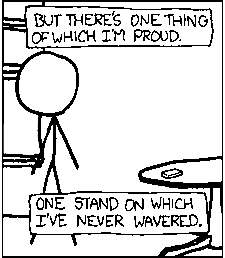
\includegraphics[width=3cm]{bilder/ringtone_2.png}\\\vspace{35mm}
        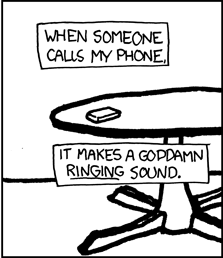
\includegraphics[width=3cm]{bilder/ringtone_3.png}\\\vspace{35mm}
    }
}
\paragraph{Die FSK-Sitzung}

Die unabhängigen Fachschaften koordinieren sich in Heidelberg universitätsweit in der \gls{FSK}\footnote{\url{www.fachschaftskonferenz.de}}, Eurer Studierendenvertretung an der Hochschule und darüber hinaus. Sie agiert mit ständiger Rückkopplung zur Basis der Studierenden und unabhängig von parteipolitischen Interessen. Ihr gehören als stimmberechtigte Mitglieder alle aktiven Fachschaften an. Die \gls{FSK} tagt im Semester jede zweite Woche öffentlich am Dienstag um 19.00 Uhr \gls{s.t.} in den Räumen des Zentralen Fachschaftenbüros (ZFB), Albert-Überle-Straße 3-5. JedeR kann hinkommen und mitreden.

Vier Hauptfunktionen nimmt die \gls{FSK}"=Sitzung wahr:
\begin{enumerate}
\item die Fachschaften koordinieren sich untereinander
\item die hochschul"= und allgemeinpolitischen Aktivitäten von Referaten und Arbeitskreisen werden diskutiert, geplant und ggf. beschlossen
\item die Arbeit der \gls{FSK}-VertreterInnen in offiziellen Gremien wird koordiniert
\item es wird über die Verwendung von Geldern zur Förderung studentischer Aktivität (z.B. Unterstützung für Theatergruppen, etc.) entschieden.
\end{enumerate}

Darüber hinaus unterstützt die \gls{FSK}, auf Antrag, auch viele unterschiedliche studentische Gruppen organisatorisch und finanziell. Von \gls{FSK}"=Mitteln wird außerdem die Zeitung UNiMUT gedruckt, die auch online\footnote{\url{http://unimut.fsk.uni-heidelberg.de/aktuell/}} zu finden ist.

Die eigentliche fachbereichsübergreifende Arbeit der \gls{FSK} läuft über Referate, Arbeitskreise und AGs, an denen ihr ebenfalls einfach teilnehmen könnt. Diese befassen sich mit übergreifenden Themen wie Studienreform, Verfasste Studierendenschaft, Qualität der Lehre, BAföG, Öffentlichkeitsarbeit oder EDV. Ergebnisse und Anregungen aus dieser Arbeit bringen sie in die \gls{FSK} ein. Während die Arbeitskreise inhaltlich unabhängiger sind, sind ReferentInnen, genau wie \gls{FSK}-VertreterInnen in Gremien, der \gls{FSK} rechenschaftspflichtig und setzen in ihrer Arbeit die Beschlüsse der \gls{FSK} um.

In Kooperation mit Studierendenvertretungen anderer Hochschulen in der Landesstudierendenvertretung, durch Öffentlichkeitsarbeit und Aktionen bemüht sich die \gls{FSK} um Durchsetzung studentischer Interessen.

Tagesordnungen und Protokolle der \gls{FSK}-Sitzung sind für alle Studierenden auf der Homepage der Fachschaftskonferenz einsehbar.

\paragraph{Arbeitsbereiche und Referate}

Die \gls{FSK} und die Fachschaften arbeiten in vielen Bereichen, zum Beispiel:

\vspace{-0.6\baselineskip}
\begin{itemize}
 \addtolength{\itemsep}{-0.6\baselineskip}
 \item Fachschaftsvernetzung und -koordination
 \item Unterstützung studentischer Gruppen
 \item landes- und bundesweite studentische Politik
 \item Erstsemestereinführungen
 \item Studentische Studienberatung
 \item Lehramtsbildung
 \item Kommunales, z.B. Straßenbahn durchs Neuenheimer Feld
 \item Gremienarbeit, z.B. in den Fakultätsräten, im Senat, beim Studentenwerk
 \item Studienreform
\end{itemize}

Koordiniert wird die Arbeit in den zuständigen Referaten:

\vspace{-0.6\baselineskip}
\begin{itemize}
 \addtolength{\itemsep}{-0.6\baselineskip}
 \item EDV-Referat
 \item Sozialreferat
 \item Antidiskriminierungs-Referat
 \item Referat für Kommunales und Verkehr
 \item Kultur- und Sportreferat
 \item Referat für Ökologie und Nachhaltigkeit 
 \item Referat für Finanzen und Internes
 \item Referat für Öffentlichkeitsarbeit \& Agitation
 \item Referat für Studienreform und hochschulpolitische Entwicklungen
 \item Referat für Politische Bildung und Vernetzung
\end{itemize}

Sämtliche Referate und Arbeitskreise der FSK freuen sich über Studis, die Interesse haben, sich in den entsprechenden Themen einzubringen und mitzuarbeiten! Die Kontaktdaten der Referate und Arbeitskreise findet ihr auf der Homepage der \gls{FSK}.
